%\documentclass{beamer}
\documentclass[handout]{beamer}

\usepackage{pgfpages} 

%\setbeameroption{show only notes}

\usetheme{default}

\mode<presentation> {
%  \usetheme{Warsaw}
  \usetheme{Frankfurt}
%  \usetheme{Boadilla}
%  \usetheme{Marburg}
}

\mode<handout>{\setbeamercolor{background canvas}{bg=black!5} %
    \pgfpagesuselayout{4 on 1}[letterpaper,border shrink=4mm,landscape] %
    \setbeameroption{show notes}}

\title[CAC Intro] {TeraGrid}
\author{Brock Palen\\ \texttt{brockp@umich.edu}}
\date{TBD}

\begin{document}
  \setbeamercovered{transparent}  
  \begin{frame}
    \titlepage
    \url{http://cac.engin.umich.edu/teragrid/}
  \end{frame}

%table of contents
  \begin{frame}{Outline}
    \tableofcontents
  \end{frame}
  
  \section{About}
  \subsection {About}
  \begin{frame}{TeraGrid}
   \begin{block}{About}
    TeraGrid is an open scientific discovery infrastructure combining leadership class resources at eleven partner sites to create an integrated, persistent computational resource.
   \end{block}
   \begin{block}{Short Form}
    \begin{itemize}
     \item<2-> Lots of Compute
     \item<3-> Lots of Storage
     \item<4-> Powerful Support
    \end{itemize}
   \end{block}
  \end{frame}

  \begin{frame}{Support}
   \begin{block}{Local Support}
    \begin{itemize}
     \item The CAC is the campus-wise local resource for TeraGrid support, and U of M user advocate on TG
     \item \url{tg-support@umich.edu}
     \item \url{http://cac.engin.umich.edu/teragrid/}
    \end{itemize}
   \end{block}
   \begin{block}{TG Wide}
    \begin{itemize}
     \item \url{help@teragrid.org}
     \item \url{http://teragrid.org/userinfo/}
    \end{itemize}
   \end{block}
  \end{frame}

  \section{Resources}
  
  \subsection{Compute}
  \begin{frame}{Resources}
   \begin{block}{Compute}
    \begin{itemize}
      \item Over 16 Compute (Batch) systems available
      \item Range from 0.34 TFlops to 608 TFlops
      \item Special resources such as GPU's and Cell CPUs available
      \item Shared memory, Distributed memory clusters, and Grid systems
    \end{itemize}
   \end{block}
  \end{frame}

  \begin{frame}{Hardware Examples}
   \begin{center}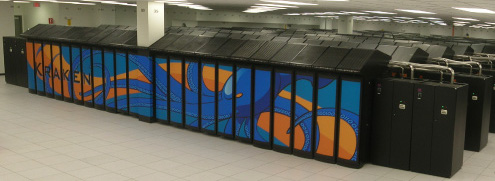
\includegraphics[height=1.5in]{kraken}\end{center}
   \begin{block}{NICS Kraken}
    \begin{itemize}
     \item CRAY XT5
     \item 66,048 AMD CPUs
     \item PGI Compilers
     \item 2.4 PetaByte Scratch Disk
    \end{itemize}
   \end{block}
  \end{frame}
 
  \begin{frame}{Hardware Examples}
   \begin{center}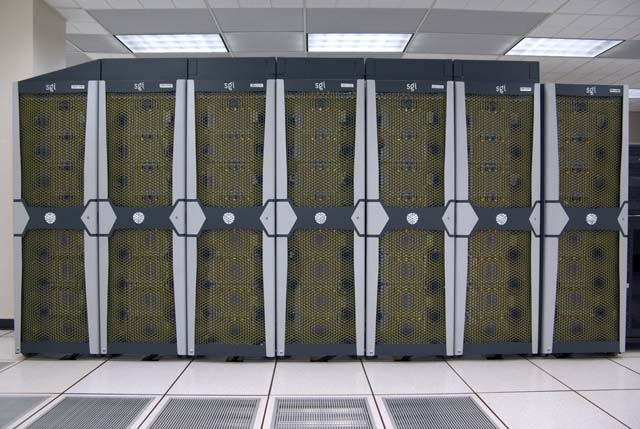
\includegraphics[height=1.80in]{pople}\end{center}
   \begin{block}{PSC Pople}
    \begin{itemize}
     \item SGI Altix 4700
     \item 768 Intel Itanium II's
     \item Intel Compilers
     \item 1.54Tbytes Shared Memory
    \end{itemize}
   \end{block}
  \end{frame}


  \subsection{Storage and Vis}
  \begin{frame}{Resources}
   \begin{block}{Storage}
     \begin{itemize}
      \item Each site/system has local scratch and NFS/Lustre home directories.
      \item Each site/system has own quota/purge policy
      \item Archive storage (Longterm/huge storage) is available at several sites, most are over 1PetaByte in size
     \end{itemize}
   \end{block}
   \begin{block}{Visualization}
   \begin{itemize}
    \item TeraGrid also gives access to several Vis clusters and walls
    \item Not as easy to use due to location but is available
   \end{itemize}
   \end{block}
  \end{frame}

  \section{Getting Allocations}
  \begin{frame}{Allocations}
    Submit all requests via POPS: \\
    \url{https://pops-submit.teragrid.org/}
   \begin{block}{Startup/Education Allocations}
    \begin{itemize}
     \item Up-to 200,000 Service Units (SUs)
     \item Up to 5TB Disk and 25TB Tape/Archive
     \item Granted all year long, for quick turn around, and startups
    \end{itemize}
   \end{block}
   \begin{block}{Research Allocations}
    \begin{itemize}
     \item Allocations larger than Startups
     \item Granted at intervals during the year
     \item Requires formal proposal
    \end{itemize}
     \url{http://teragrid.org/userinfo/access/allocations.php}
   \end{block}
  \end{frame}

  \subsection{Starup Allocations}

  \begin{frame}{Starup/Education Allocations}
   \begin{block}{Startup Requirements}
    \begin{itemize}
     \item Granted all year long
     \item Use to make formal proposal for Research Allocation
      \begin{itemize}
       \item Define goals 
       \item Discover target system
       \item Estimate number of needed SU's
      \end{itemize}
     \item Easier request process requiring a curriculum vitae and abstract 
    \end{itemize}
   \end{block}
   \begin{block}{Details on Starup Allocations}
    \url{http://teragrid.org/userinfo/access/dac.php}
   \end{block}
  \end{frame}

  \subsection{Research Allocations}

  \begin{frame}{Research Allocations}
   \begin{block}{Research Requirements}
    \begin{itemize}
     \item For those who need more than the Startup Allocation
     \item Allocations start January 1, April 1, July 1, and October 1
     \item Requests are submitted in September, December, March, and June
     \item Requires formal request to TeraGrid
    \end{itemize}
   \end{block}
   \begin{block}{Tips for Writing a Request}
    \url{http://teragrid.org/userinfo/access/allocations.php\#writing}
   \end{block}
  \end{frame}
\end{document}
